\documentclass{article}

% Language setting
% Replace `english' with e.g. `spanish' to change the document language
\usepackage[spanish]{babel}

% Set page size and margins
% Replace `letterpaper' with `a4paper' for UK/EU standard size
\usepackage[letterpaper,top=2cm,bottom=2cm,left=3cm,right=3cm,marginparwidth=1.75cm]{geometry}

% Useful packages
\usepackage{amsmath}
\usepackage{graphicx}
\usepackage{enumitem}
\usepackage{comment}
\usepackage{wrapfig}
\usepackage[colorlinks=true, allcolors=blue]{hyperref}

\title{AED Tema 3. Árboles II: estructuras para búsqueda}
\author{Martín González Dios 
\href{https://github.com/martindios}{\includegraphics[height=0.5cm]{github.png}}}

\begin{document}
\maketitle

\section{Árboles binarios de búsqueda (ABB)}
\subsection{Definición}
\begin{itemize}
    \item \textbf{Dado un nodo}: todos los datos del subárbol izquiero son menores, todos los datos del subárbol derecho son mayores.

    \item \textbf{Clave de ordenación}: criterio de ordenación menor - mayor.

    \item Ventaja: \textbf{tiempo de ejecución promedio O(log(N))}. Pero es necesario imponer condiciones de balanceado (árbole AVL, árboles B, etc) sobre los ABB para que se mantenga O(log(N)), ya que si no balanceamos en el peor caso O(N) de tiempo de ejecución.

    \item Recorrido inorden (IRD): datos de menor a mayor.
\end{itemize}

\begin{figure}[h]
    \centering
    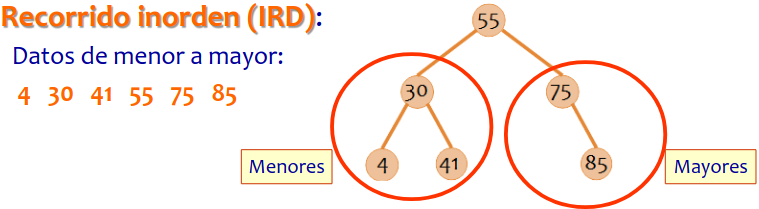
\includegraphics[width=0.7\textwidth]{img-t3/img_193_37.png}
\end{figure}

\subsection{Inserción}
En un ABB la inserción no se puede realizar en el primer hueco libre que se vea, sino que hay que \textbf{respetar la estructura}, buscando desde la raíz el hueco correspondiente al nodo que queremos insertar. Por tanto, la inserción es recursiva, ya que se parte del nodo raíz y se va mirando si el elemento que queremos insertar es menor o mayor, bajando por la rama correspondiente hasta encontrar su sitio. \\

Como clara \textbf{desventaja} de este tipo de árbol tenemos el caso en el que la mayor parte de los elementos que se inserten sean mayores mayores o menores que el nodo raíz, provocando un \textbf{árbol desbalanceado}, lo que aumenta el tiempo de búsqueda al tener que recorrer muchos elementos.

\subsection{Eliminación}
La desventaja en el caso de la eliminación reside en tener que \textbf{reestructurar el árbol si se eliminan ciertos nodos}, para mantener la estructura que cumpla las restricciones de los ABB.
\begin{enumerate}
    \item Si el \textbf{nodo es hoja}, se suprime del árbol sin más.
    \item Si el nodo tiene \textbf{un único hijo}, se intercambia de posición con su hijo y se elimina del árbol.
    
    \item Si el \textbf{nodo tiene dos hijos}, buscamos el menor de todos los descendientes del hijo derecho, sustituimos por dicho nodo, y lo eliminamos del árbol. Otra opción es sustituir por el nodo de mayor valor de los descendientes del subárbol izquierdo.
\end{enumerate}

\section{Árboles parcialmente ordenados o montículos}
Es un \textbf{árbol binario completo parcialmente ordenado}: \\
Completo: en el nivel más bajo pueden faltar algunos nodos, pero éstos han de ser los más a la derecha posibles. \\
Parcialmente ordenado, existen 2 tipos: \\
\begin{itemize}
    \item \textbf{Montículo de mínimos}: clave nodo $\leq$ clave hijos (padre $<$ que hijos).

    \item \textbf{Montículo de máximos}: clave nodo $\geq$ clave hijos (padre $>$ que hijos).
\end{itemize}

\subsection{Propiedades del montículo binario o heap}
\begin{itemize}
    \item Da soporte eficiente a los \textbf{operadores del TAD cola de prioridad}, que proporciona una flexibilidad extra a la hora de ordenar.

    \item El orden parcial es más débil que el orden total (sin embargo es más eficiente de mantener), pero más fuerte que el orden aleatorio (de manera que el elemento con mayor prioridad se puede identificar de forma rápida, ya que siempre es la raíz).
\end{itemize}

\subsection{Inserción}
Como árbol binario completo que es, la inserción se hace en el \textbf{hueco libre más a la izquierda de su último nivel}. Sin embargo, si se inserta un \textbf{elemento} con un valor (para este ejemplo considérese montículo de mínimos) \textbf{menor que su padre}, es necesario \textbf{reorganizar el árbol} intercambiando el elemento con su padre hasta llegar a una posición en la que se cumpla el criterio.

\subsection{Eliminación}
En este tipo de árboles, el elemento que se quiere \textbf{suprimir es siempre el de mayor prioridad}, es decir, \textbf{la raíz}. Para llevar a cabo esta operación, el nodo raíz se intercambia de posición con el nodo hoja más a la derecha (el nodo más a la derecha del último nivel), y una vez allí, se elimina. A continuación, se procede a la reorganización del nuevo nodo raíz hasta encontrar su sitio, intercambiándolo con (en nuestro caso) el hijo menor en cada caso.

\subsection{Monticulización (Heapify)}
Proceso en el que dado un conjunto de elementos, nos pedirán \textbf{representarlos por medio de un montículo} (de máximos o de mínimos).

\begin{enumerate}
    \item \textbf{Dibujar el árbol} que resulta a partir del array.
    \item Si el árbol tiene L niveles, \textbf{desde i = L - 1 hasta 1}:
    \begin{itemize}
        \item Comprobar si cada nodo de nivel i cumple la \textbf{regla de orden parcial}. Si no la cumple intercambiar con el menor/mayor de sus hijos.
        \item \textbf{Propagar esta comprobación} hacia los niveles desde i hasta L - 1.
    \end{itemize}
\end{enumerate}


\begin{comment}
\begin{figure}[h]
    \centering
    \includegraphics[width=0.5\textwidth]{1.png}
\end{figure}
\end{comment}

\begin{comment}
\begin{wrapfigure}[]{r}{0.5\linewidth}
    \centering
    \includegraphics[width=\linewidth]{8.png}
\end{wrapfigure}
\end{comment}

\end{document}